\section{Сверхбыстрые полностью оптические переключатели}

Одним из ключевых строительных элементов схем управления светом являются оптические переключатели, позволяющие контролировать распространение света в волноводах. Точно так же, как реле оказались весьма ограниченно применимыми в электронных микросхемах и были вытеснены транзисторами, существующие оптомеханические переключатели являются слишком медленными и габаритными для использования их в фотонных микросхемах. Для выполнения логических операций требуются сверхбыстрые и полностью управляемые светом оптические переключатели. При этом желательно, чтобы подобные схемы полностью состояли из кремния, как материала, доминирующего в микроэлектронной индустрии, что является довольно сложной задачей из-за относительно слабых нелинейных свойств кремния.

Первый кремниевая структура, способная работать в режиме сверхбыстрого полностью оптического переключателя была представлен в работе \cite{Vilson2004}. Структура представляла из себя волновод с расположенным рядом кольцевым резонатором (рисунок \ref{fig:ring}). Спектр пропускания связанного с резонатором волновода изображён на рисунке \ref{fig:ring_spectrum}. В подобной схеме свет, первоначально распространявшийся в волноводе, захватывается резонатором и повторно интерферирует с сигналом. Была показана способность управлять коэффициентом преломления кольца путём освещения его лазерным пучком и инжекции свободных носителей посредством механизма двухфотонного поглощения. Изменения в коэффициенте преломления сдвигали резонансную частоту и позволяли управлять распространением светового пучка в волноводе.

\begin{figure}[h]
	\begin{subfigure}[b]{.53\textwidth}
		\centering
		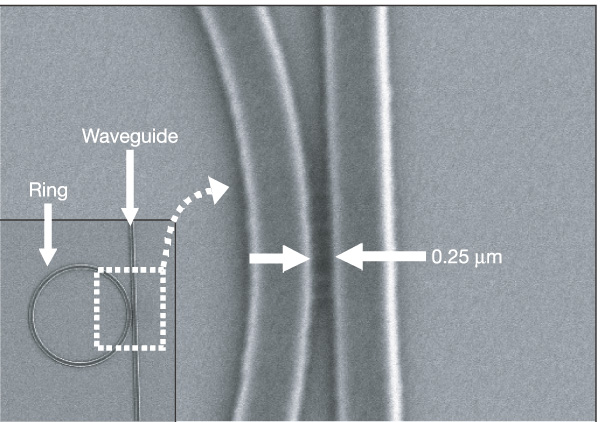
\includegraphics[width=.9\textwidth]{img/ring}
		\caption{Кольцевой резонатор}
		\label{fig:ring}
	\end{subfigure}
	\begin{subfigure}[b]{.47\textwidth}
		\centering
		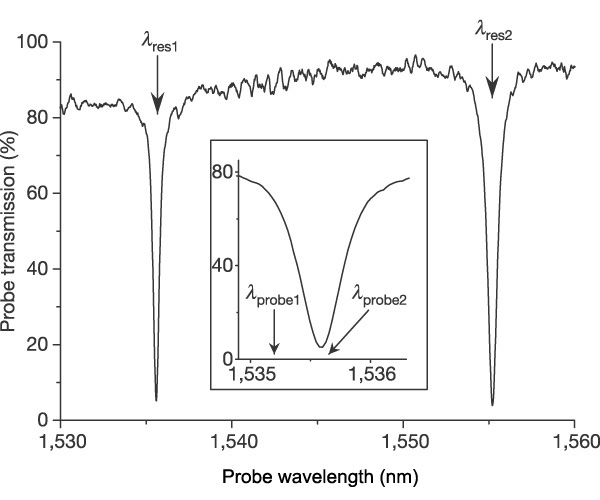
\includegraphics[width=.9\textwidth]{img/ring_spectrum}
		\caption{Спектр пропускания волновода}
		\label{fig:ring_spectrum}
	\end{subfigure}
	\caption{}
\end{figure}

Аналогичные по функционалу структуры были также показаны в работах \cite{Kippenberg2004, Gondarenko2009, Pollinger2009, Soltani2007}.